\section{Adding Noise}\label{P1}

This section involves the addition of various noises to the image, 
followed by the development of filters and their application to the noisy image 
in order to evaluate its performance. In order to accompany the presentation of this report, 
one of the images has been selected. 
The image in question has been subjected to the application of Gaussian noise with 
a standard deviation of twenty, as well as salt and pepper noise with a density of twenty percent. 
It is possible to view the original image as well as the photos with various noises, along with 
their respective histograms, displayed in Figure 1. 
It is necessary to define two distinct local functions in MATLAB for the purpose of adding 
these noises to the images. These functions are for Gaussian noise and Salt-Pepper noise, 
respectively. After that, these routines can be invoked in order to introduce noise 
into the photos.
Taking into consideration the images that are displayed together with their histograms 
in Figure 1, it is clear that the photos have undergone significant transformations and 
appear to be quite noisy. An appropriate filter ought to be developed in order to eliminate 
these disturbances while yet preserving the necessary features of the photos.

\begin{figure} [ht]
    \centering
    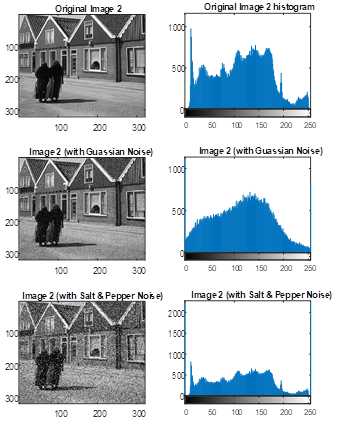
\includegraphics[scale = 1.5, angle=0]{Resources/Images_Org_Nosied.png}
    \caption{Original Image, Image with Gaussian noise, and Image with Salt \& pepper noise and their histograms}
    \label{fig:AddingNoise}
\end{figure}